\documentclass[letterpaper]{article}
\usepackage[margin=1in]{geometry}
\usepackage[utf8]{inputenc}
\usepackage{textcomp}
\usepackage{amssymb}
\usepackage{natbib}
\usepackage{graphicx}
\usepackage{gensymb}
\usepackage{amsthm, amsmath, mathtools}
\usepackage[dvipsnames]{xcolor}
\usepackage{enumerate}
\usepackage{mdframed}
\usepackage[most]{tcolorbox}
\usepackage{csquotes}
% https://tex.stackexchange.com/questions/13506/how-to-continue-the-framed-text-box-on-multiple-pages

\tcbuselibrary{theorems}

\newcommand{\R}{\mathbb{R}}
\newcommand{\Z}{\mathbb{Z}}
\newcommand{\N}{\mathbb{N}}
\newcommand{\Q}{\mathbb{Q}}
\newcommand{\C}{\mathbb{C}}
\newcommand{\code}[1]{\texttt{#1}}
\newcommand{\mdiamond}{$\diamondsuit$}
\newcommand{\PowerSet}{\mathcal{P}}
\newcommand{\Mod}[1]{\ (\mathrm{mod}\ #1)}
\DeclareMathOperator{\lcm}{lcm}

%\newtheorem*{theorem}{Theorem}
%\newtheorem*{definition}{Definition}
%\newtheorem*{corollary}{Corollary}
%\newtheorem*{lemma}{Lemma}
\newtheorem*{proposition}{Proposition}


\newtcbtheorem[number within=section]{theorem}{Theorem}
{colback=green!5,colframe=green!35!black,fonttitle=\bfseries}{th}

\newtcbtheorem[number within=section]{definition}{Definition}
{colback=blue!5,colframe=blue!35!black,fonttitle=\bfseries}{def}

\newtcbtheorem[number within=section]{corollary}{Corollary}
{colback=yellow!5,colframe=yellow!35!black,fonttitle=\bfseries}{cor}

\newtcbtheorem[number within=section]{lemma}{Lemma}
{colback=red!5,colframe=red!35!black,fonttitle=\bfseries}{lem}

\newtcbtheorem[number within=section]{example}{Example}
{colback=white!5,colframe=white!35!black,fonttitle=\bfseries}{def}

\newtcbtheorem[number within=section]{note}{Important Note}{
        enhanced,
        sharp corners,
        attach boxed title to top left={
            xshift=-1mm,
            yshift=-5mm,
            yshifttext=-1mm
        },
        top=1.5em,
        colback=white,
        colframe=black,
        fonttitle=\bfseries,
        boxed title style={
            sharp corners,
            size=small,
            colback=red!75!black,
            colframe=red!75!black,
        } 
    }{impnote}
\usepackage[utf8]{inputenc}
\usepackage[english]{babel}
\usepackage{fancyhdr}
\usepackage[hidelinks]{hyperref}

\pagestyle{fancy}
\fancyhf{}
\rhead{CSE 105}
\chead{Monday, January 03, 2022}
\lhead{Lecture 1}
\rfoot{\thepage}

\setlength{\parindent}{0pt}

\begin{document}

\section{Mathematical Notions and Terminology}
Here, we will review several topics from discrete mathematics. 

\subsection{Sets and Subsets}
Throughout this class, we will be using the concept of sets, tuples, and more. We begin with sets. 

\subsubsection{Sets}
\begin{definition}{Set}{}
    A \textbf{set} is a collection of objects represented as a unit.
\end{definition}
Sets may contain any type of objects, including numbers, symbols, and even other sets. The objects in a set are called its \textbf{elements} or \textbf{members}. For example, consider the set:
\[S = \{7, 21, 57\}\]
The set $S$ contains 3 elements. To indicate set membership or nonmembership, we use $\in$ and $\notin$, respectively. So, $7 \in S$ means that 7 \emph{is in} $S$ while $8 \notin S$ means that 8 \emph{is not in} $S$. 

\bigskip 

Additionally, we note that the order of describing a set doesn't matter, nor does reptition of its members. So, the set $A = \{1, 2, 3\}$ and $Z = \{2, 1, 3\}$ are exactly the same; that is $A = Z$. A generalization of a set that does allow for duplicates does exist, though (see multisets).  

\bigskip

Several other common examples of sets are:
\begin{itemize}
    \item \textbf{Singleton sets}, or sets that contain one element. For example, $\{5\}$ is a singleton set. 
    \item \textbf{Empty set}, or sets that contain no elements. These are written $\emptyset$. It should be noted that $\{\emptyset\} \neq \emptyset$!
    \item \textbf{Unordered pair}, or sets that contain two elements. For example, $\{5, 2\}$ is an unordered pair because $\{5, 2\} = \{2, 5\}$. 
\end{itemize}

\subsubsection{Defining Sets}

There are two main ways to define a set. 
\begin{itemize}
    \item Explicitly writing out the elements. For example, the set $S$ of all positive integers between 1 and 5 can be written like so: 
    \[S = \{2, 4\}\]

    \item Through a rule. Generally, to describe a set containing elements that adhere to a rule, we use:
    \[\{n \mid \text{Rule about } n\}\]
    So, for example, the example used in the previous bullet point could have been written like so: 
    \[S = \{n \mid 1 < n < 5 \text{ and } n = 2m \text{ for some } m \in \Z\}\]
\end{itemize}

\subsubsection{Subsets}

\begin{definition}{Subset}{}
    A set $A$ is called a \textbf{subset} of a set $B$, written $A \subseteq B$, if every member of $A$ is also a member of $B$. 
\end{definition}
For example, the set $A = \{7\}$ is a \emph{subset} of $S$ since $7 \in A$ and $7 \in S$. However, the set $B = \{7, 8\}$ is \emph{not a subset} of $S$ since $7 \in B$ and $7 \in S$ \emph{but} $8 \in B$ while $8 \notin S$. 

\begin{definition}{Proper Subset}{}
    A set $A$ is called a \textbf{proper subset} of a set $B$, written $A \subset B$ or $A \subsetneq B$, if $A$ is a subset of $B$ and is not equal to $B$. 
\end{definition}
So, for example, the set $A = \{7, 21\}$ is a proper subset of $S$, written $A \subsetneq S$, since every element in $A$ is in $S$ but both aren't equal. However, the set $A = \{7, 21, 57\}$ is not a proper subset of $S$. 

\subsubsection{Multisets}

\begin{definition}{Multiset}{}
    A \textbf{multiset} is a generalization of a set that allows for multiple instances for each of its elements. 
\end{definition}
For example, define $X = \{1, 1, 2, 3\}$ and $Z = \{1, 2, 3\}$. Then, $X$ and $Z$ are precisely the same as \emph{sets} but are different as \emph{multisets}. However, note that order still doesn't matter; for example, $\{1, 1, 2, 3\}$ and $\{1, 2, 1, 3\}$ are still the same \emph{multisets}. 

\subsubsection{Infinite Sets}

\begin{definition}{Infinite Set}{}
    An \textbf{infinite set} is a set that contains infinitely many elements.
\end{definition}
Several common examples of infinite sets are $\Z$ (the set of all integers), $\N$ (the set of all positive integers), $\R$ (the set of all real numbers). 

\subsubsection{Union, Intersections, and Complements}

\begin{definition}{Union}{}
    The \textbf{union} of two sets $A$ and $B$, written $A \cup B$, is the set we get by combining all of the elements in $A$ and $B$ into a single set. Mathematically, we write this as: 
    \[A \cup B = \{n \mid n \in A \text{ or } n \in B\}\]
\end{definition}
For example, given $A = \{1, 2\}$ and $B = \{2, 3\}$, $A \cup B = \{1, 2, 3\}$. 

\begin{definition}{Intersection}{}
    The \textbf{intersection} of two sets $A$ and $B$, written $A \cap B$, is the set we get by combining all \emph{common} elements of $A$ and $B$ into a single set. Mathematically, we write this as: 
    \[A \cap B = \{n \mid n \in A \text{ and } n \in B\}\]
\end{definition}
For example, given the same two sets $A$ and $B$ used in the union example, $A \cap B = \{2\}$. 

\begin{definition}{Complement}{}
    The \textbf{complement} of a set $A$ is the set of all elements that are not in $A$.
\end{definition}
For example, consider the set $E$ of all even integers. Then, the complement of $E$ is the set of all odd integers.

\subsubsection{Power Set}
\begin{definition}{Power Set}{}
    The \textbf{power set} of $A$, denoted $\mathcal{P}(A)$ is the set of all subsets of $A$.
\end{definition}
For example, if $A$ is the set $\{0, 1\}$, then $\mathcal{P}(A)$ would be: 
\[\{\emptyset, \{0\}, \{1\}, \{0, 1\}\}\] 

\subsection{Sequences and Tuples}
Here, we will review sequences and tuples (kind of like ordered sets).

\subsubsection{Sequences}
\begin{definition}{Sequence}{}
    A \textbf{sequence} of objects is a list of these objects in some order.
\end{definition}
We usually write a sequence by writing the objects within parentheses. For example, the sequence 7, 21, 57 would be written:
\[(7, 21, 57)\]
As implied, the order \underline{matters} in a sequence. In other words, the sequence $(7, 21, 57)$ is not the same as $(57, 7, 21)$. Additionally, repetition \underline{matters} in a sequence. So, $(7, 21, 57)$ is not the same sequence as $(7, 21, 21, 57)$. 

\subsubsection{Tuples}
\begin{definition}{Tuple}{}
    A finite sequence is often called a \textbf{tuple}. A sequence with $k$ elements is a \textbf{$k$-tuple}.
\end{definition}
So, $(7, 21, 57)$ is a 3-tuple. As a side note, a 2-tuple is also called an \textbf{ordered pair}.

\subsubsection{Cartesian Product}
\begin{definition}{Cartesian Product}{}
    The \textbf{Cartesian product} of two sets $A$ and $B$, written $A \times B$, is the set of all ordered pairs wherein the first element is a member of $A$ and the second element is a member of $B$. 
\end{definition}
If $A = \{1, 2\}$ and $B = \{x, y\}$, then:
\[A \times B = \{(1, x), (1, y), (2, x), (2, y)\}\]

\begin{definition}{Extended Cartesian Product}{}
    The \textbf{Cartesian product} of $k$ sets, $A_1, A_2, \dots, A_k$, written $A_1 \times A_2 \times \dots \times A_k$, is the set of all $k$-tuples $(a_1, a_2, \dots, a_k)$ where $a_i \in A_i$ for $1 \leq i \leq k$. 
\end{definition}
Using the definition of $A$ and $B$ from the previous definition, it follows that: 
\[A \times B \times A = \{(1, x, 1), (1, x, 2), (1, y, 1), (1, y, 2), (2, x, 1), \dots\}\]
If we have the Cartesian product of a set $A$ with itself, we can use the shorthand: 
\[\underbrace{A \times \dots \times A}_{k \text{ times}} = A^k\]
Another (familiar) example is $\R \times \R$, or the set of all real points. We can define this set like so: 
\[\{(i, j) \mid i, j \in R\}\]
Some example and non-example of elements are: 
\[(1, 5) \in \R \times \R\]
\[\left(\frac{1}{2}, \sqrt{2}\right) \in \R \times \R\]
\[(-0.8213, -92.3) \in \R \times \R\]
\[(i, 3 + 2i) \notin \R \times \R\]


\subsection{Functions}
A function is an object that sets up an input-output relationship. In other words, a function takes an input and produces an output. In every function, the same input always produces the same output. So, if $f$ is a function whose output value is $b$ when the input value is $a$, we write:
\[f(a) = b\]
Alternatively, a function is called a \textbf{mapping}. In other words, for the above function definition, we say that $f$ maps $a$ to $b$. 

\begin{definition}{Function Definitions}{}
    For a function $f: A \mapsto B$:
    \begin{itemize}
        \item The \textbf{domain} $A$ is the set of possible inputs to the function.
        \item The \textbf{codomain} $B$ is the set of possible output values\footnote{The book states that the range is the set of output values, but later states that the function may not use all the elements in the range.}. 
        \item The \textbf{range} is the set of actual output values. This is a subset of $B$.
    \end{itemize}
\end{definition}
Consider the function $\text{abs}: \R \mapsto \R$ defined by:
\[\text{abs}(x) = |x|\]
Here, the domain is the set of all real numbers. The codomain is the set of all real numbers as well. However, the range is the set of all \emph{non-negative} real numbers, that is, $\R_{\geq 0}$.

\subsubsection{Cartesian Product Input}
The domain of a function $f$ can be the Cartesian product of multiple sets $A_1 \times \dots \times A_k$ for some sets $A_1, \dots, A_k$. In this case, $f$'s input is a $k$-tuple $(a_1, \dots, a_k)$ where $a_i$ are the \textbf{arguments} to $f$. In this case, the function with $k$-arguments is called a \textbf{$k$-ary function} and $k$ is called the \textbf{arity} of the function. Note that:
\begin{itemize}
    \item If $k = 1$, then $f$ has a single argument and $f$ is called a \textbf{unary function}.
    \item If $k = 2$, $f$ is a \textbf{binary function}. 
\end{itemize}
Certain binary functions can be written in a special \textbf{infix notation}; for example, the function:
\[\text{add}: \R \times \R \mapsto \R\] 
Is often written as $a + b$ (with the $+$ symbol between the two arguments) instead of the \textbf{prefix notation} (with symbol preceding) $\text{add}(a, b)$. 

\subsubsection{Predicates}
\begin{definition}{Predicate}{}
    A \textbf{predicate} is a function whose range is $\{\text{true}, \text{false}\}$. 
\end{definition}
For example, the function:
\[\text{even}: \Z \mapsto \{\text{true}, \text{false}\}\] 
Takes in an integer and outputs \code{true} if the integer is even and \code{false} otherwise. So: 
\[\text{even}(10) = \text{true}\]
\[\text{even}(11) = \text{false}\]
A predicate whose domain is a set of $k$-tuples $A \times \dots \times A$ is called a \textbf{relation}, a $k$-\textbf{ary} relation, or a \textbf{$k$-ary relation on $A$}. A common case is a 2-ary relation, called a \textbf{binary relation}, for which we often use infix notation. For example, several very common binary relations are the ``less than'' and ``equals'' relation. 

\bigskip

If $R$ is a binary relation, then the statement $aRb$ means that $aRb$ is \code{true}. For example, if $R$ is the binary relation $<$, then $3 < 5$ is \code{true}. Similarly, if $R$ is a $K$-ary relation, the statement $R(a_1, \dots, a_k)$ means that $R(a_1, \dots, a_k)$ is \code{true}.

\subsubsection{Equivalence Relations}
Suppose $R$ is a relation over a set $S$. Then:
\begin{itemize}
    \item $R$ is called \textbf{reflexive} if $\forall x \in S$, $x R x$. That is, every $x \in S$ is related to itself. 
    \item $R$ is called \textbf{symmetric} if $\forall x, y \in S$, $x R y \implies y R x$. In other words, if $x$ is related to $y$, is $y$ related to $x$? 
    \item $R$ is called \textbf{transitive} if $\forall x, y, z \in S$, $x R y$ and $y R z$ implies that $x R z$. 
\end{itemize}

For example, define the equivalence relation on $\N$, written $\equiv_7$. For any $i, j, k \in \N$, say $i \equiv_7 j$ if $i - j$ is a multiple of 7. This is an equivalence relation because: 
\begin{itemize}
    \item It is reflexive as $i - i = 0$ and 0 is a multiple of 7. 
    \item It is symmetric as $i - j$ is a multiple of 7 if $j - i$ is a multiple of 7. 
    \item It is transitive as whenever $i - j$ and $j - k$ are both multiples of 7, then $i - k = (i - j) + (j - k)$ is the sum of two multiples of 7, and hence a multiple of 7.  
\end{itemize}


\subsection{Undirected Graphs}
\begin{definition}{Undirected Graph}{}
    An \textbf{undirected graph}, or simply a \textbf{graph} is a pair $G = (V, E)$, where:
    \begin{itemize}
        \item $V$ is a set whose elements are called \emph{nodes} or \emph{vertices}.
        \item $E$ is a set of paired nodes, whose elements are called \emph{edges}.
    \end{itemize} 
    Informally, an undirected graph is a set of points with lines connecting some of these points. The points are called nodes or vertices and the lines are called edges.  
\end{definition}
In an \underline{undirected} graph $G$ that contains nodes $i$ and $j$, the pair $(i, j)$ or $(j, i)$ represents the edge that connects $i$ and $j$; in other words, $(i, j)$ and $(j, i)$ are the same. So, it follows that the order in which we put $i$ and $j$ in the tuple doesn't matter. Because order doesn't matter, we may also represent $(i, j)$ as $\{i, j\}$.

\bigskip

For example, the following graph is an undirected graph:
\begin{center}
    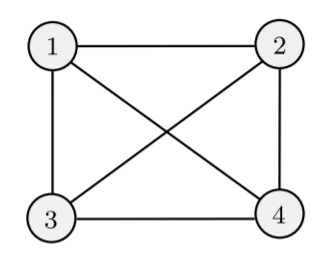
\includegraphics[scale=0.7]{../assets/rectangle_graph.png}
\end{center}

\begin{definition}{Degree of a Node}{}
    The number of edges at a particular node is the \textbf{degree} of that node. 
\end{definition}
We note that no more than one edge is allowed between any two nodes; however, we may allow an edge from a node to itself (called a \emph{self-loop}). 

\bigskip

Looking at the graph above, we can define $G = (V, E)$ where\footnote{Remember, because we're working with an undirected graph, an edge like $(1, 2)$ and $(2, 1)$ refer to the same edge!}:
\begin{itemize}
    \item $V = \{1, 2, 3, 4\}$
    \item $E = \{(1, 2), (1, 3), (1, 4), (2, 3), (2, 4), (3, 4)\}$
\end{itemize}
Additionally, each node has degree 3 because each node has 3 edges.  

\subsubsection{Labeled Graph}
A graph is a \textbf{labeled graph} if the nodes and/or edges of a graph are labeled. For example, we might represent each node as a city and each edge as the number of miles from node A to node B. 

\subsubsection{Subgraph}
\begin{definition}{Subgraph}{}
    A graph $G$ is a \textbf{subgraph} of graph $H$ if the nodes of $G$ are a subset of the nodes of $H$ \emph{and} the edges of $G$ are the edges of $H$ on the corresponding nodes.
\end{definition}
In other words, if we had $G = (V', E')$ and $H = (V, E)$, we must have:
\begin{itemize}
    \item $V' \subseteq V$
    \item $E' \subseteq E$
\end{itemize}
The following figure shows a graph $H$ and a subgraph $G$:
\begin{center}
    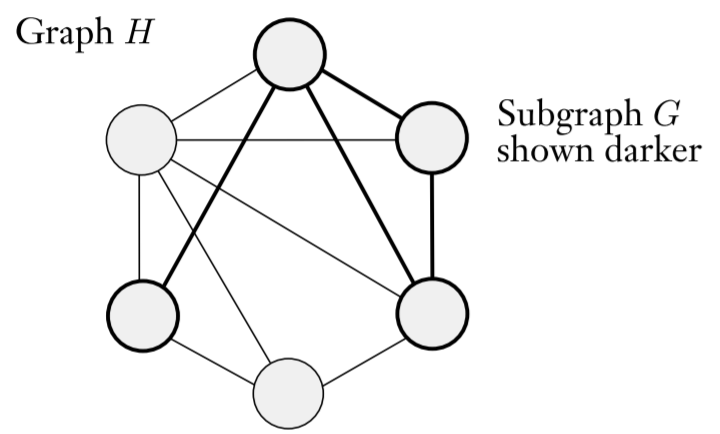
\includegraphics[scale=0.5]{../assets/subgraph.png}
\end{center}

\subsubsection{Path}
\begin{definition}{Path}{}
    A \textbf{path} in a graph is a sequence of nodes connected by edges. 
\end{definition}
For example, a path might look like: 
\begin{center}
    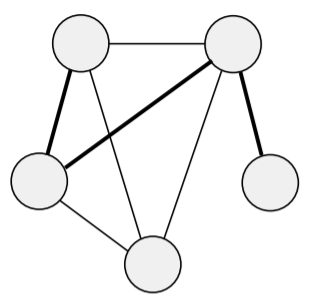
\includegraphics[scale=0.5]{../assets/path.png}
\end{center}

\begin{definition}{Simple Path}{}
    A \textbf{simple path} is a path that doesn't repeat any nodes. 
\end{definition}

\subsubsection{Connections Between Nodes}
\begin{definition}{Connected Graph}{}
    A graph is \textbf{connected} if every two nodes have a path between them. 
\end{definition}
So, the graph in the above example is a connected graph. 

\begin{definition}{Cycles}{}
    A path is a \textbf{cycle} if it starts and ends in the same node.
\end{definition}
For example, a cycle might look like: 
\begin{center}
    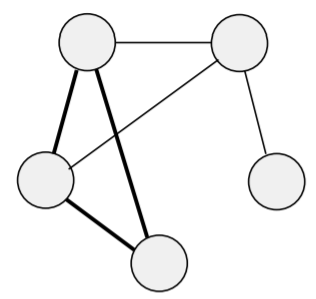
\includegraphics[scale=0.5]{../assets/cycle.png}
\end{center}

\begin{definition}{Simple Cycle}{}
    A \textbf{simple cycle} is a cycle that contains at least three nodes and repeats only the first and last node.
\end{definition}

\subsubsection{Trees}
\begin{definition}{Tree}{}
    A graph is a \textbf{tree} if it is connected and has no simple cycles. 
\end{definition}
A tree can contain a specially designated node called the \emph{root}, which is usually a singular node at the ``top'' that branches out to every other node. In this case, the nodes of degree 1 in a tree, other than the root, are called the \emph{leaves} of the tree. 

\bigskip

A tree might look like: 
\begin{center}
    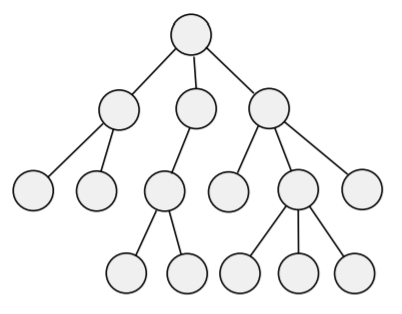
\includegraphics[scale=0.42]{../assets/tree.png}
\end{center}


\subsection{Directed Graphs}
\begin{definition}{Directed Graph}{}
    A \textbf{directed graph} is a pair $G = (V, E)$ where: 
    \begin{itemize}
        \item $V$ is a set whose elements are called \emph{nodes} or \emph{vertices}.
        \item $E$ is a set of paired nodes, whose elements are called \emph{directed edges}.
    \end{itemize}
    Informally, a directed graph is a set of points with \underline{arrows} instead of lines connecting some of these points. 
\end{definition}
In a \underline{directed} graph that contains nodes $i$ and $j$, the pair $(i, j)$ and $(j, i)$ \textbf{do not represent} the same edges. In particular, $(i, j)$ means that there is an arrow pointing \emph{from} $i$ to $j$; then, $(j, i)$ means that there is an arrow pointing from $j$ to $i$. In other words, the order \textbf{does} matter. 

\bigskip

For example, the following graph is a directed graph:
\begin{center}
    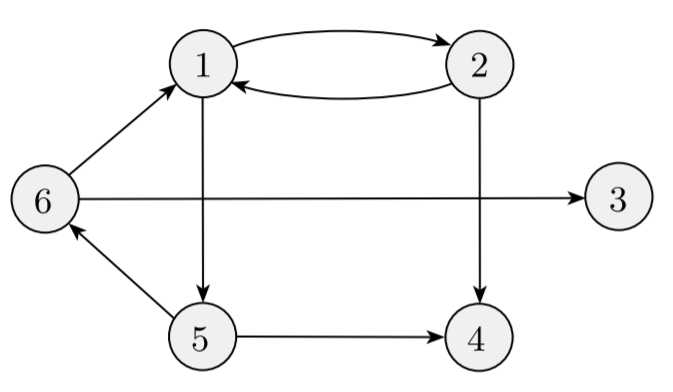
\includegraphics[scale=0.5]{../assets/directed_graph.png}
\end{center}
We can define $G = (V, E)$ as: 
\begin{itemize}
    \item $V = \{1, 2, 3, 4, 5, 6\}$
    \item $E = \{(1, 2), (2, 1), (6, 1), (6, 3), (1, 5), (2, 4), (5, 4), (5, 6)\}$
\end{itemize}

\subsubsection{Directed Path}
\begin{definition}{Directed Path}{}
    A path in which all the arrows point in the same direction as its steps is called a \textbf{directed path}. 
\end{definition}

\subsubsection{Connections}
\begin{definition}{}{}
    A directed graph is \textbf{strongly connected} if a directed path connects every two nodes.
\end{definition}

\subsubsection{Relationship to Binary Relations}
We can use directed graphs to depict binary relations. In particular, if $R$ is a binary relation whose domain is $D \times D$, a labeled graph $G = (D, E)$ represents $R$, where $E = \{(x, y) \mid xRy\}$. For example, for $D = \{1, 2, 3\}$ and binary relation $<$, the edges would be: 
\[E = \{(1, 2), (2, 3), (1, 3)\}\]



\newpage 
\section{Boolean Logic}
Boolean logic is a mathematical system built around \code{true} and \code{false}, which are often represented as \code{1} and \code{0}, respectively. We can manipulate boolean values with boolean operations. The operations are as follows:
\begin{description}
    \item[Negation:] The negation, or \textbf{not}, operation is designated with the symbol $\neg$. The negation of a Boolean value is simply the opposite value. Therefore: 
    \begin{center}
        \begin{tabular}{c|c}
            $a$ & $\neg a$ \\ 
            \hline 
            0 & 1 \\ 
            1 & 0
        \end{tabular}
    \end{center}
    
    \item[Conjunction:] The conjunction, or \textbf{and}, operation is designated with the symbol $\land$. The conjunction of two Boolean values is 1 if both values are 1 and 0 otherwise.
    \begin{center}
        \begin{tabular}{c c|c}
            $a$ & $b$ & $a \land b$ \\ 
            \hline 
            0 & 0 & 0 \\ 
            0 & 1 & 0 \\ 
            1 & 0 & 0 \\ 
            1 & 1 & 1
        \end{tabular}
    \end{center}

    \item[Disjunction:] The disjunction, or \textbf{or}, operation is designated with the symbol $\lor$. The disjunction of two Boolean values is 1 of either of those values are 1 and 0 otherwise.   
    \begin{center}
        \begin{tabular}{c c|c}
            $a$ & $b$ & $a \lor b$ \\ 
            \hline 
            0 & 0 & 0 \\ 
            0 & 1 & 1 \\ 
            1 & 0 & 1 \\ 
            1 & 1 & 1
        \end{tabular}
    \end{center} 
\end{description}

There are several other operators that may occasionally appear; they are: 
\begin{description}
    \item[Exclusive OR:] The \emph{exclusive or}, or \textbf{XOR}, is designated by $\oplus$; it is 1 if either, but not both, of the operands is 1. 
    \begin{center}
        \begin{tabular}{c c|c}
            $a$ & $b$ & $a \oplus b$ \\ 
            \hline 
            0 & 0 & 0 \\ 
            0 & 1 & 1 \\ 
            1 & 0 & 1 \\ 
            1 & 1 & 0
        \end{tabular}
    \end{center} 

    \item[Equality:] The \emph{equality} operator is designated by $\longleftrightarrow$; it is 1 if both operands have the same value. 
    \begin{center}
        \begin{tabular}{c c|c}
            $a$ & $b$ & $a \longleftrightarrow b$ \\ 
            \hline 
            0 & 0 & 1 \\ 
            0 & 1 & 0 \\ 
            1 & 0 & 0 \\ 
            1 & 1 & 1
        \end{tabular}
    \end{center} 
    
    \item[Implication:] The \emph{Implication} operator is designated by $\longrightarrow$; it is 0 if its first operand is 1 and its second operand is 0 and 1 otherwise. 
    \begin{center}
        \begin{tabular}{c c|c}
            $a$ & $b$ & $a \longrightarrow b$ \\ 
            \hline 
            0 & 0 & 1 \\ 
            0 & 1 & 1 \\ 
            1 & 0 & 0 \\ 
            1 & 1 & 1
        \end{tabular}
    \end{center} 
\end{description}

Finally, the \textbf{distributive law} for \code{AND} and \code{OR} is useful when manipulating Boolean expressions. That is: 
\[P \land (Q \lor R) = (P \land Q) \lor (P \land R)\]
\[P \lor (Q \land R) = (P \lor Q) \land (P \lor R)\]





\newpage 
\section{Strings and Languages}
\begin{definition}{Alphabet}{}
    An \textbf{alphabet} is any nonempty finite set. Generally, we use $\Sigma$ and $\Gamma$ to designate alphabets.
\end{definition}

\begin{definition}{Symbols}{}
    The members of the alphabet are the \textbf{symbols} of the alphabet.
\end{definition}

Some example of alphabets are: 
\[\Sigma_1 = \{\code{0, 1}\}\]
\[\Sigma_2 = \{\code{a, b, c, d, e, f, g, h, i, j, k, l, m, n, o, p, q, r, s, t, u, v, w, x, y, z}\}\]
\[\Gamma = \{\code{0, 1, x, y, z}\}\]

\begin{definition}{String}{}
    A \textbf{string} over an alphabet is a finite sequence of symbols from that alphabet, usually written next to one another and not separated by commas. 
\end{definition}
For example, if we use $\Sigma_1$ as our alphabet, then \code{01001} is a \textbf{string} over $\Sigma_1$. Likewise, if we use $\Sigma_2$ as our alphabet, then \code{something} is a string over $\Sigma_2$. 

\bigskip

The set of all finite strings over $\Sigma$ (any general alphabet) is denoted by $\Sigma^*$. Here, this includes:
\begin{itemize}
    \item The empty string $\epsilon$.
    \item Any \textbf{finite} combination of the symbols in this alphabet.
\end{itemize}
This does not include infinite sequences of symbols. It does have infinitely many elements. 

\bigskip

So, for example, $\Sigma_{1}^{*}$ would have strings like (and keep in mind that these are just examples): 
\[\epsilon \in \Sigma_{1}^{*} \qquad \code{0} \in \Sigma_{1}^{*} \qquad \code{1} \in \Sigma_{1}^{*}\]
\[\code{010101} \in \Sigma_{1}^{*} \qquad \code{1111} \in \Sigma_{1}^{*} \qquad \code{0000} \in \Sigma_{1}^{*}\]

\begin{definition}{Length}{}
    If $w$ is a string over $\Sigma$, then the \textbf{length} of $w$, written $|w|$, is the number of symbols that it contains. 
\end{definition}
\textbf{Remarks:}
\begin{itemize}
    \item The string of length zero is called the \textbf{empty string} and is written $\epsilon$. The empty string plays the role of 0 (like an identity) in a number system.
    \item If $w$ has length $n$, then we can write $w = w_1 w_2 \dots w_n$ where each $w_i \in \Sigma$.
\end{itemize} 

\begin{definition}{Reverse}{}
    The \textbf{reverse} of a string $w$, written $w^{\mathcal{R}}$, is the string obtained by writing $w$ in the opposite order.
\end{definition}
\textbf{Remark:} In other words, for a string $w$, we can write the reverse of $w$ as $w^{\mathcal{R}} = w_n w_{n - 1} \dots w_{2} w_{1}$. 

\begin{definition}{Substring}{}
    A string $z$ is a \textbf{substring} of a string $w$ if $z$ appears consecutively within $w$.
\end{definition}
For example, if we look at the string $w = \code{something}$, then $z_1 = \code{some}$ and $z_2 = \code{thing}$ are both substrings of $w$. 

\begin{definition}{Concatenation}{}
    For a string $x$ of length $m$ and a string $y$ of length $n$, the \textbf{concatenation} of $x$ and $y$, written $xy$, is the string obtained by appending $y$ to the end of $x$, as in: 
    \[x_1 \dots x_m y_1 \dots y_n\]
    If we want to concatenate a string $x$ with itself many times, we use the superscript notation $x^k$ to mean: 
    \[\underbrace{xx \dots x}_{k}\]
\end{definition}
If we consider the two substrings $z_1$ and $z_2$ in the previous example, then $z_1 z_2 = \code{something}$. 

% Lexicographic Order example?

\begin{definition}{Prefix}{}
    A string $x$ is a \textbf{prefix} of a string $y$ if a string $z$ exists where $xz = y$.
\end{definition}
For example, if we look at the two substrings $z_1$ and $z_2$ in the previous example yet again, we say that $z_1$ is a prefix of $w$ since $z_1 z_2 = w$. 

\begin{definition}{Proper Prefix}{}
    A string $x$ is a proper prefix of a string $y$ if, in addition to $x$ being a prefix of $y$, $x \neq y$.
\end{definition}
So, \code{some} is a proper prefix of \code{something} while \code{something} is not a proper prefix of \code{something}.

\begin{definition}{Language}{}
    A \textbf{language} is a set of strings. 
\end{definition}

\begin{definition}{Prefix-Free}{}
    A language is \textbf{prefix-free} if no member is a proper prefix of another member.
\end{definition}













\newpage 
\section{Finite Automata (1.1)}
Consider the controller for an automatic one-way door.
\begin{center}
    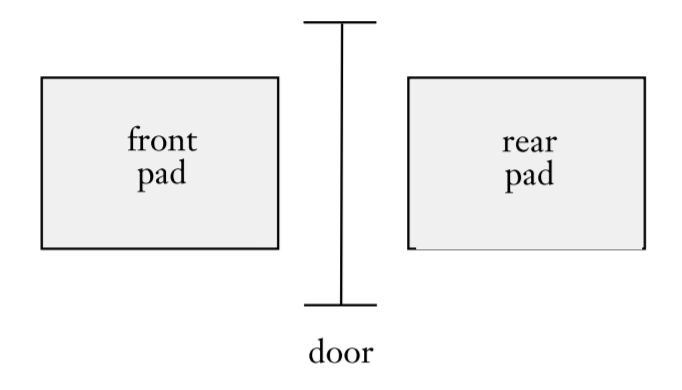
\includegraphics[scale=0.4]{../assets/door.png}
\end{center}
Here:
\begin{itemize}
    \item The front pad is there is to detect the presence of a person who is about to walk through the doorway. 
    \item The rear pad is there so that the controller can hold the door open long enough for the person to pass all the way through while also ensuring that no one behind door is hit by the door. 
\end{itemize}
The controller is in either of two states: \code{OPEN} or \code{CLOSED}. This represents the condition of the door. There are also \emph{four} possible input conditions: 
\begin{itemize}
    \item \code{FRONT}: A person is standing on the pad in front of the doorway (the front pad).
    \item \code{REAR}: A person is standing on the pad to the rear of the doorway (the rear pad).
    \item \code{BOTH}: People are standing on both pads. 
    \item \code{NEITHER}: No one is standing on either pad.
\end{itemize}
The corresponding state diagram is: 
\begin{center}
    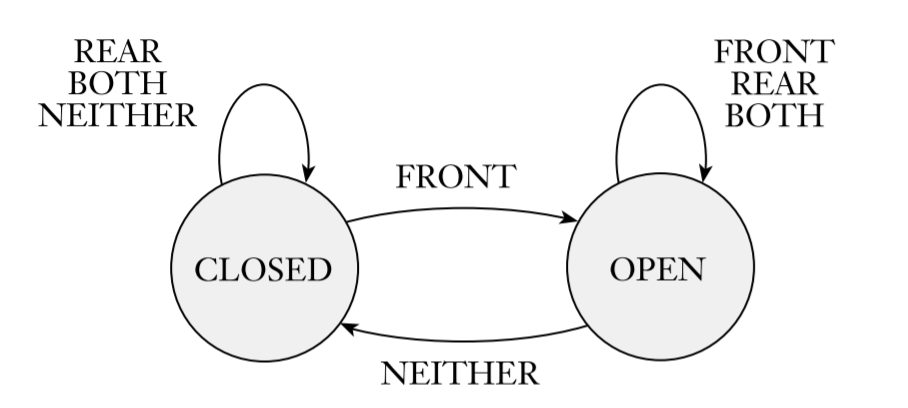
\includegraphics[scale=0.4]{../assets/door_state.png}
\end{center}
And the corresponding transition table: 
\begin{center}
    \begin{tabular}{c|c c c c} 
                & \code{NEITHER} & \code{FRONT} & \code{REAR} & \code{BOTH} \\ 
            \hline
            \code{CLOSED} & \code{CLOSED} & \code{OPEN} & \code{CLOSED} & \code{CLOSED} \\ 
            \code{OPEN} & \code{CLOSED} & \code{OPEN} & \code{OPEN} & \code{OPEN} 
    \end{tabular}
\end{center}

The controller moves from state to state depending on what input it receives. For example: 
\begin{itemize}
    \item When it starts off in the \code{CLOSED} state and receives input \code{NEITHER} or \code{REAR}, it remains in the \code{CLOSED} state. In the state diagram, if we start at the \code{CLOSED} circle (state), both \code{NEITHER} and \code{REAR} loop back to \code{CLOSED}.
    \item Again, when the controller is in the \code{CLOSED} state and it receives the \code{BOTH} input, then it stays in the \code{CLOSED} state because opening the door may knock someone over on the rear pad (as the door opens towards the rear side).
    \item If the controller is in the \code{OPEN} state, then receiving the inputs \code{FRONT}, \code{REAR}, or \code{BOTH} will result in the controller remaining \code{OPEN}. However, if it receives the \code{NEITHER} input, then it goes to a \code{CLOSED} state. 
\end{itemize}
Essentially, \textbf{for the state diagram}, start at the initial state (circle) and follow the arrow depending on what input signals are received. \textbf{For the transition table}, look at the row corresponding to the initial state and the column corresponding to the input; the resulting cell will be the new state of the controller.

\bigskip

The figures used above (the state diagram and transition table) are both standard ways of representating a finite automaton. While this door may be very simple (due to the fact that it only really needs to store an extremely small amount of memory), in reality, we may be dealing with other devices with somewhat more memory. 

\bigskip

Both finite automata and their probablistic counterpart \textbf{Markov chains} are useful tools when we want to attempt to recognize patterns in data. 

\subsection{From a Mathematical Perspective}
Consider the following figure, which depicts a finite automaton called $M_1$:
\begin{center}
    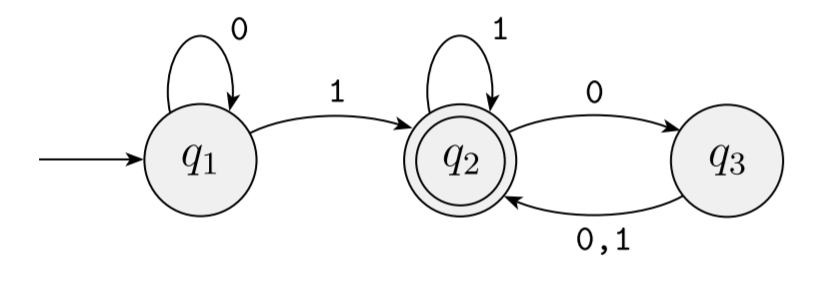
\includegraphics[scale=0.4]{../assets/finite_automaton_1.png}
\end{center}
There are a few things to note here: 
\begin{itemize}
    \item The above figure for $M_1$ is called the \textbf{state diagram} of $M_1$. 
    \item $M_1$ has three \textbf{states}, labeled $q_1$, $q_2$, and $q_3$. 
    \item The \textbf{start state} is the state indicated by the arrow pointing at it from nowhere. In the case of the above state diagram, this would be $q_1$. 
    \item The \textbf{accept state} is the state with a \underline{double circle}. In the case of the above state diagram, this would be $q_2$. 
    \item The \textbf{transitions} are the arrows going from one state to another. 
\end{itemize}
For a given input string, \underline{this} automaton processes that string and produces an output that is either \code{ACCEPT} or \code{REJECT}. For this automaton, the processing works like so: 
\begin{enumerate}
    \item Here, the processing begins in $M_1$'s start state. 
    \item Then, the automaton receives the symbols from the input string one by one from left to right. 
    \item After reading each symbol, $M_1$ moves from one state to another along the transition that has that symbol as its label. 
    \item When it reads the last symbol, $M_1$ produces its output. The output is \code{ACCEPT} if $M_1$ is now in an accept state and \code{REJECT} if it is not. 
\end{enumerate}
As an example, suppose we give $M_1$ the input string \code{1101}. Then, the processing proceeds as follows: 
\begin{itemize}
    \item Start in state $q_1$. 
    \item Read \code{1}. Transition from $q_1$ to $q_2$. 
    \item Read \code{1}. Transition from $q_2$ to $q_2$. 
    \item Read \code{0}. Transition from $q_2$ to $q_3$. 
    \item Read \code{1}. Transition from $q_3$ to $q_2$. 
    \item \code{ACCEPT} because $M_1$ is in an accept state $q_2$ at the end of the input. 
\end{itemize}
So, really, what matters is that we \emph{end up} at the accept state. 

\subsection{Formal Definition of a Finite Automaton}
A finite automaton has several parts.
\begin{itemize}
    \item It has a set of states and rules for going from one state to another, depending on the input symbol.
    \item It has an input alphabet that indicates the allowed input symbols. 
    \item It has a start state and a set of accept states. 
\end{itemize}
We use something called a \textbf{transition function}, often denoted $\delta$, to define the rules for moving. If the finite automaton has an arrow from a state $x$ to a state $y$ labeled with the input symbol \code{1}, that means that if the automaton is in state $x$ when it reads a \code{1}, it then moves to state $y$. We can indicate the same thing with the transition function by saying that: 
\[\delta(x, \code{1}) = y\]
All of this leads to the formal definition:
\begin{definition}{Finite Automaton}{}
    A \textbf{finite automaton} is a 5-tuple $(Q, \Sigma, \delta, q_0, F)$ where: 
    \begin{enumerate}
        \item $Q$ is a finite set called the \textbf{states}.
        \item $\Sigma$ is a finite set called the \textbf{alphabet}.
        \item $\delta: Q \times \Sigma \mapsto Q$ is the \textbf{transition function}.
        \item $q_0 \in Q$ is the \textbf{start state}.
        \item $F \subseteq Q$ is the \textbf{set of accept states} (sometimes also called \emph{final states}).
    \end{enumerate}
\end{definition}
\textbf{Remark:} $F$ can be the empty set $\emptyset$, which means that there are 0 accept states.

\subsection{Applying the Definition}
Consider again $M_1$:
\begin{center}
    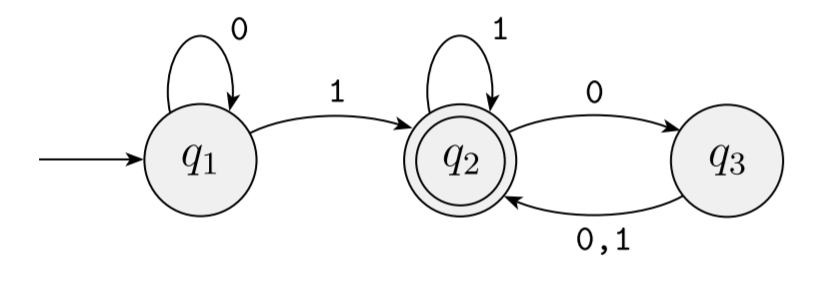
\includegraphics[scale=0.4]{../assets/finite_automaton_1.png}
\end{center}
Using the formal definition above, we can describe $M_1$ formally be writing $M_1 = (Q, \Sigma, \delta, q_1, F)$, where: 
\begin{itemize}
    \item $Q = \{q_1, q_2, q_3\}$
    \item $\Sigma = \{\code{0, 1}\}$
    \item $\delta$ is defined as: 
    \begin{center}
        \begin{tabular}{c|c c}
                  & \code{0} & \code{1} \\ 
            \hline 
            $q_1$ & $q_1$    & $q_2$ \\ 
            $q_2$ & $q_3$    & $q_2$ \\ 
            $q_3$ & $q_2$    & $q_2$ 
        \end{tabular}
    \end{center}
    \item $q_1$ is the start state. 
    \item $F = \{q_2\}$. 
\end{itemize}

\subsection{Machine and Language}
If $A$ is the set of all strings (i.e. language) that machine $M$ accepts, we say that $A$ is the \textbf{language of machine} $M$, write $L(M) = A$, and say that $M$ recognizes $A$. 

\bigskip

A machine may accept \emph{several strings}, but it always recognizes \underline{one language}. A machine can accept no strings; in this case, it still recognizes the empty language $\emptyset$. 

\bigskip

If we consider our example automaton $M_1$, then define: 
\[A = \{w \mid w \text{ contains at least one \code{1} or an even number of \code{0}s follow the last \code{1}}\}\]
Which means that $L(M_1) = A$, of equivalently, $M_1$ recognizes $A$. 

\subsubsection{Example 1: Simple Finite Automaton}
Consider the following state diagram for the finite automaton $M_2$:
\begin{center}
    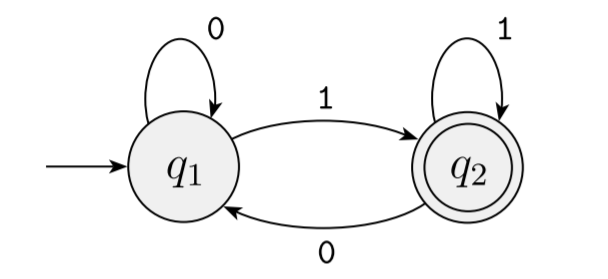
\includegraphics[scale=0.4]{../assets/finite_automaton_2.png}
\end{center}
Here, the formal description of $M_2$ is as follows: 
\[M_2 = (\{q_1, q_2\}, \{\code{0, 1}\}, \delta, q_1, \{q_2\})\]
Where $\delta$ is: 
\begin{center}
    \begin{tabular}{c|c c}
            & \code{0} & \code{1} \\
        \hline  
        $q_1$ & $q_1$ & $q_2$ \\ 
        $q_2$ & $q_1$ & $q_2$
    \end{tabular}
\end{center}
To figure out what $A$ is, we try a few different strings.
\begin{center}
    \begin{tabular}{c|c}
        \textbf{String Input} & \textbf{Output} \\ 
        \hline 
        $\epsilon$ & \code{REJECT} \\ 
        \code{1} & \code{ACCEPT} \\ 
        \code{0} & \code{REJECT} \\ 
        \code{01} & \code{ACCEPT} \\ 
        \code{10} & \code{REJECT} \\ 
        \code{11} & \code{ACCEPT}
    \end{tabular}
\end{center}
It's quite clear that $A$ is simply the set of all strings that end with \code{1}. So:
\[A = \{w \mid w \text{ ends with \code{1}.}\}\]

\subsubsection{Example 2: Finite Automaton}
Consider the following state diagram for the finite automaton $M_3$:
\begin{center}
    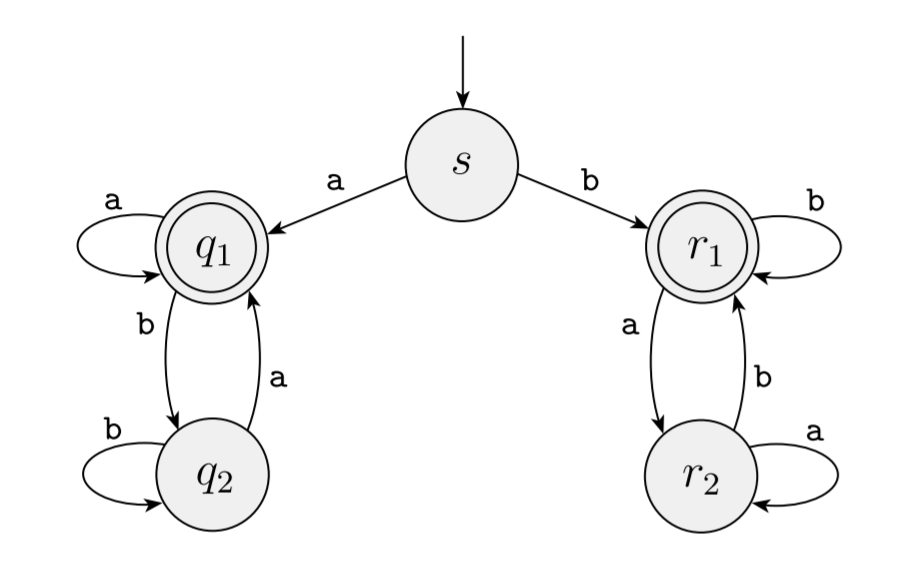
\includegraphics[scale=0.4]{../assets/finite_automaton_3.png}
\end{center}
Here, the formal description of $M_3$ is as follows: 
\[M_3 = (\{s, q_1, q_2, r_1, r_2\}, \{\code{a, b}\}, \delta, s, \{q_1, r_1\})\]
Where $\delta$ is: 
\begin{center}
    \begin{tabular}{c|c c}
            & \code{a} & \code{b} \\
        \hline  
        $s$  & $q_1$ & $r_1$ \\ 
        $q_1$ & $q_1$ & $q_2$ \\ 
        $q_2$ & $q_1$ & $q_2$ \\ 
        $r_1$ & $r_2$ & $r_1$ \\ 
        $r_2$ & $r_2$ & $r_1$ \\
    \end{tabular}
\end{center}
Here, we note that we cannot end at the start state. In other words, when we start with \code{a}, we take the left branch to $q_1$. In the left branch, notice how when we end with \code{a}, we will always end up at $q_1$, the accept state. So, it follows that a string like the one below is acceptable: 
\[\code{a}w_2 w_3 \dots w_{n - 1} \code{a} \qquad w_i \in \{\code{a, b}\}\]
Likewise, if we start with \code{b}, we take the right branch to $r_1$. In the right branch, if our string ends with \code{b}, we will always end up at $r_1$. So, it follows that a string like the one below is also acceptable:
\[\code{b}w_2 w_3 \dots w_{n - 1} \code{b} \qquad w_i \in \{\code{a, b}\}\]
In other words, for this automaton, a string that starts and ends with the same symbol is accepted. That is: 
\[A = \{w \mid w \text{ starts and ends with the same symbol.}\}\]

\subsubsection{Example 3: Complicated Finite Automaton}
Sometimes, it is hard to describe a finite automaton by state diagram. In this case, we may end up using a formal description to specify the machine. Consider the following example with the alphabet: 
\[\Sigma = \{\code{RESET, 0, 1, 2}\}\]
Where \code{RESET} is treated as one symbol. For each $i \geq 1$, define $A_i$ to be the language of all strings where the sum of the numbers is a multiple of $i$, except that the sum is reset to 0 whenever the symbol \code{RESET} appears. For each $A_i$, we have a finite automaton $B_i$ which recognizes $A_i$. We define $B_i$ formally like so: 
\[B_i = (Q_i, \Sigma, \delta_i, q_0, \{q_0\})\]
Where $Q_i = \{q_0, q_1, q_2, \dots, q_{i - 1}\}$ and the transition function $\delta_i$ is defined so that for each $j$, if $B_i$ is in $q_j$ (i.e. $B_i$ is in state $q_j$), the running sum is $j$ modulo $i$. In other words, for each $q_j$ define: 
\[\delta_{i}(q_j, \code{0}) = q_j\]
\[\delta_{i}(q_j, \code{1}) = q_k \text{  where } k = j + 1 \text{ modulo } i\]
\[\delta_{i}(q_j, \code{2}) = q_k \text{  where } k = j + 2 \text{ modulo } i\]
\[\delta_{i}(q_j, \code{RESET}) = q_0\]

\bigskip

For example, suppose we have the following state machine $B_3$ which uses the same alphabet described above:
\begin{center}
    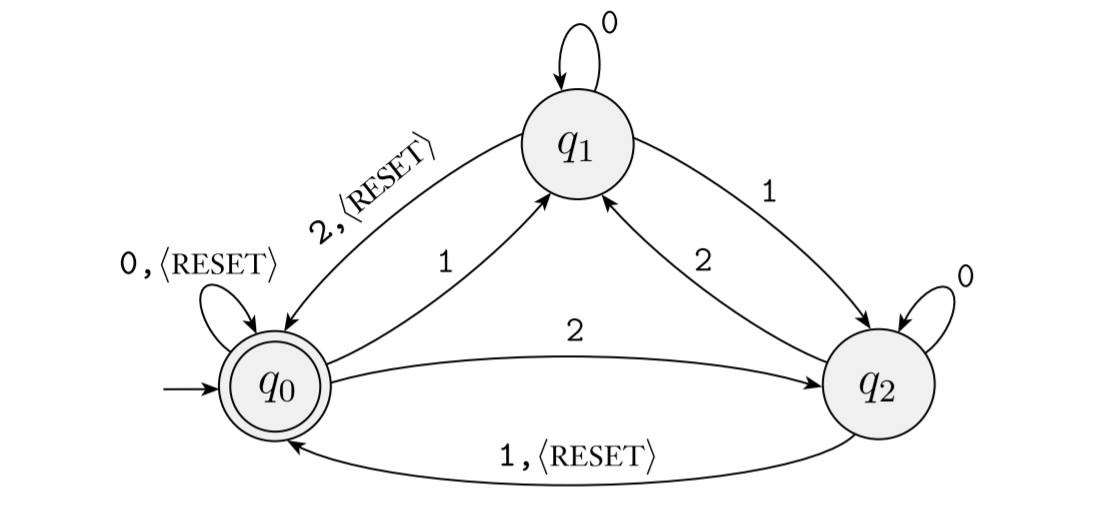
\includegraphics[scale=0.4]{../assets/finite_automaton_4.png}
\end{center}
The formal description of $B_3$ is as follows: 
\[B_3 = (\{q_0, q_1, q_2\}, \{\code{RESET, 0, 1, 2}\}, \delta, q_0, \{q_0\})\]
Where $\delta$ is defined by: 
\begin{center}
    \begin{tabular}{c|c c c c}
              & \code{RESET} & \code{0} & \code{1} & \code{2} \\
        \hline  
        $q_0$ & $q_0$        & $q_0$    & $q_1$    & $q_2$    \\ 
        $q_1$ & $q_0$        & $q_1$    & $q_2$    & $q_0$    \\
        $q_2$ & $q_0$        & $q_2$    & $q_0$    & $q_1$
    \end{tabular}
\end{center}
So, as an example, let's suppose we have the string \code{01212}. The sum of these numbers is:
\[0 + 1 + 2 + 1 + 2 = 6 \implies 6 \equiv \boxed{0} \mod{3}\]
We expect the automaton to finish at the accept state as 6 is a multiple of 3. Running through the automaton, we have: 
\begin{itemize}
    \item Input: \code{0}. Start at $q_0$, end at $q_0$.
    \item Input: \code{1}. Start at $q_0$, end at $q_1$. So, our automaton is at state $q_1$.
    \item Input: \code{2}. Start at $q_1$, end at $q_0$. So, our automaton is at state $q_0$.
    \item Input: \code{1}. Start at $q_0$, end at $q_1$. So, our automaton is at state $q_1$.
    \item Input: \code{2}. Start at $q_1$, end at $q_0$. So, our automaton is at state $q_0$.
\end{itemize}
Therefore, we are at an accept state as our string \code{01212} sums up to a multiple of 3. Of course, if there are any \code{RESET}s in our string, we can disregard everything up to and including the \emph{last} \code{RESET} as \code{RESET} puts us back at the start. That is, for instance, the string \code{0121 RESET 21011 RESET 01212} will put the state machine in the same state as \code{01212}.

\bigskip

So, it follows that our state machine recognizes the set $A_3$, which consists of all strings where all digits sum up to 0 modulo 3. That is: 
\[A_3 = \left\{w \mid \sum_{\code{d} \in w} d = 0 \Mod{3}\right\}\]
\emph{Note:} If any \code{RESET}s are in the string, we can omit everything in the string \emph{up to and including} the last \code{RESET}.

\end{document}
